\chapter{State of the Art\label{cha:chapter2}}

\section{Object Detection Methods}
State of the art object detection methods include \textit{scale invariant feature transformation} (SIFT) \cite{Lowe2004DistinctiveKeypoints}, \textit{speeded up robust features} (SURF) \cite{Bay2008Speeded-UpSURF}, \textit{binary robust invariant scalable
keypoints} (BRISK) \cite{Leutenegger2011BRISK:Keypoints}, \textit{oriented fast and rotated BRIEF} (ORB) \cite{Rublee2011ORB:SURF}, \textit{Accelerated KAZE} (AKAZE, KAZE meaning wind in Japanese) \cite{Alcantarilla2012KAZEFeatures, Alcantarilla2013FastSpaces} and \textit{template matching} (TM) \cite{Brunelli2009TemplatePractice}. The two latter shall be discussed here briefly.\newline

AKAZE feature matching is a pyramidal object detection algorithm. The Pyramidal approach declines the image ratio with every filtering step. Spanning over several scales features are detected and described. In contrast to other established algorithms like SIFT, which use a linear scale space for filtering, AKAZE instead uses a nonlinear scale space with the recently developed numerical model \textit{Fast Explicit Diffusion}. The advantage of the nonlinear scale space is depicted in figure  \ref{skalenraum}. Prominent features like edges and corners are preserved. 
\begin{figure}[ht]
	\centering
  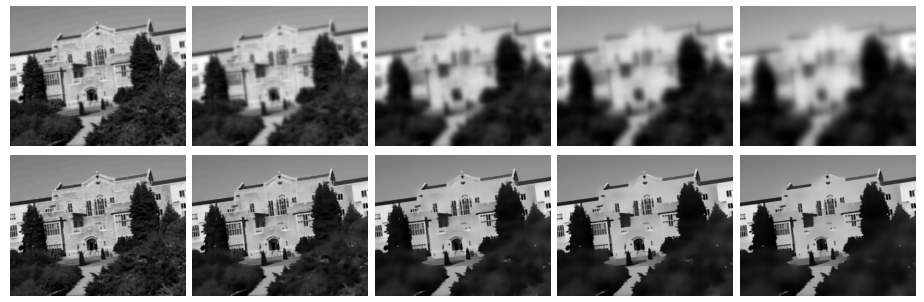
\includegraphics[width=\textwidth]{nonlinearscalespace.png}
	\caption{Top row: Gauss filtering with linear scale space and increasing standard deviation. Bottom Row: Non linear diffusion scale space. \cite{Alcantarilla2012KAZEFeatures}}
	\label{skalenraum}
\end{figure}
The outcome of AKAZE is depicted in fig \ref{AKAZE}. Matches are shown as dots connected with lines between the two pictures of the same object from another point of view.
\begin{figure}[ht]
	\centering
  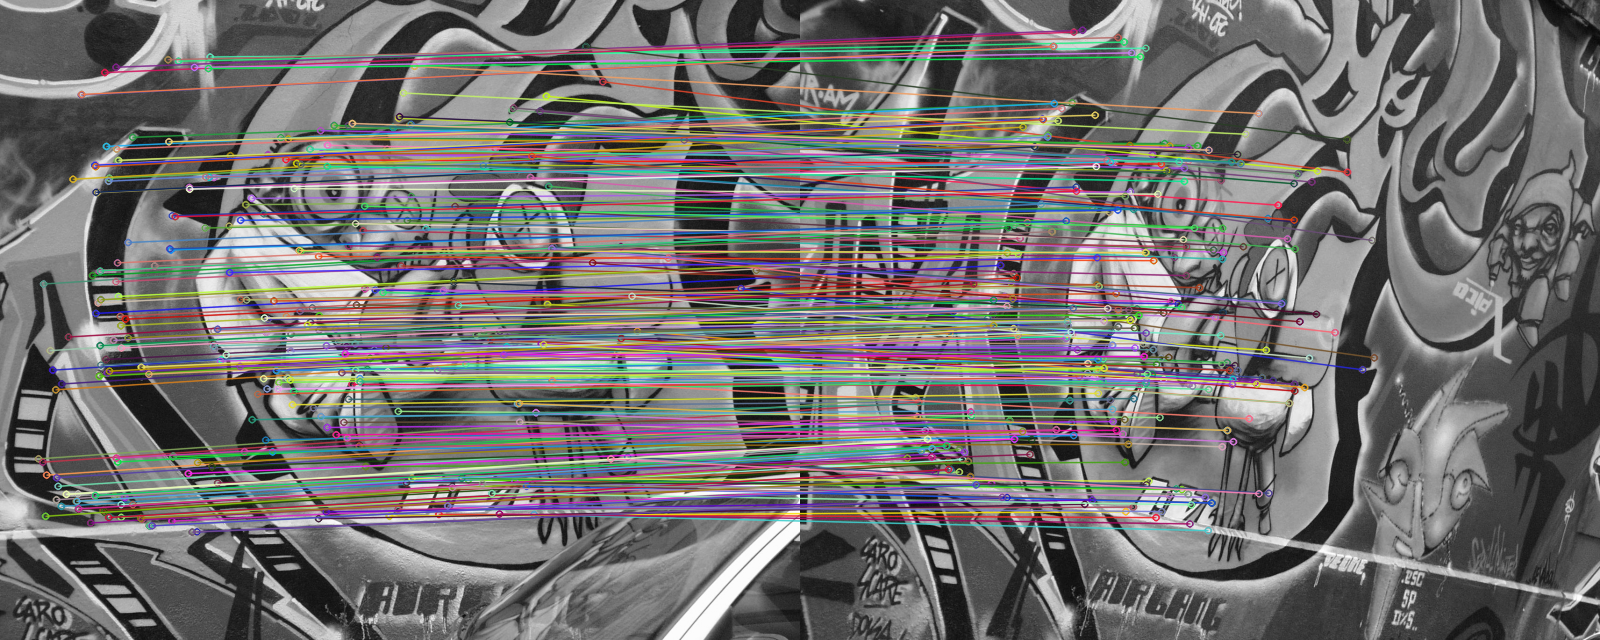
\includegraphics[width=\textwidth]{AKAZE.png}
	\caption{AKAZE Feature Matching for a grafitti viewed from two different angles. Best viewed in color. \cite{Documentation.LastVisited2018-11-15.TutorialMatching}}
	\label{AKAZE}
\end{figure}
 \newline
TM unlike AKAZE matches templates instead of features. Fig \ref{templatematching} illustrates this process. In the left image the face of the man is to be found. The template is the little cut-out in the middle. Pixel by pixel the template is being convoluted with the original image and rated with a metric. The resulting resolution matrix is depicted on the right. Bright areas indicate potential findings. At the brightest point the template is rightfully suggested.

\begin{figure}[ht]
	\centering
  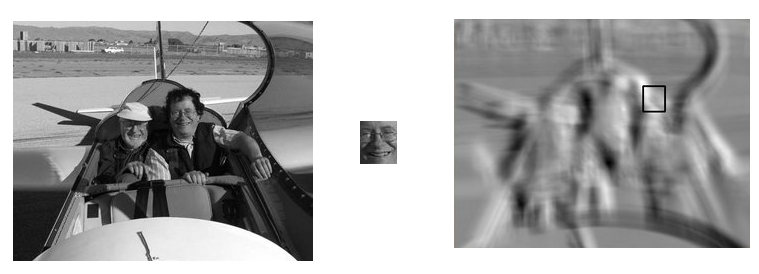
\includegraphics[width=\textwidth]{templatematching.png}
	\caption{In the picture on the left the template in the middle is to be found. Depicted on the right is the resolution matrix with potential findings indicated with the bright color and the found area of the template in the original image.\cite{Documentation.LastVisited2018-11-15.2014TemplateMatching}}
	\label{templatematching}
\end{figure}

\section {Service Interfaces}
\label{serviceinterfaces}
In this section potential client-server-based interfaces and underlying protocols for the object detection service shall be discussed. The evaluated interfaces are \textit{Advanced Message Queuing Protocol} (AMQP), \textit{message queuing telemetry transport} (MQTT), \textit{representational state transfer} (REST), \textit{Google remote procedure calls} (gRPC), \textit{graph query language} (GraphQL) and \textit{open platform communication unified architecture vision} (OPC UA Vision). \newline

Both AMQP 0.x and MQTT are broker based protocols. They are protocols specialized for machine-to-machine (M2M) communication. Clients can be sensors, programmable logic controllers etc., the server is a broker connecting the clients. A broker is a central instance mediating between parties. Clients can subscribe to various message queues called topics. Telemetry data can then be published and read from these topics handled by the broker. The clients dynamically change between publisher and subscriber. Fig \ref{MQTT} illustrates the MQTT architecture.  \cite{Banks2014MQTT3.1.1} RabbitMQ is a message broker software which supports AMQP 0.x natively and MQTT via a plugin. \cite{Lastvisited2018-15-122018WhichSupport} AMQP needs to be distinguished between 0.x and 1.0, as the underlying messaging paradigm has been completely revised. While for version 0.x strict publishing/subcription messaging is required, version 1.0 is based on a peer-to-peer connection where a broker is not required, although possible. Due to the more complex version of version 1.0, fewer implementations exist. \cite{Dizdarevic2018SurveyIntegration}

\begin{figure}[ht]
	\centering
  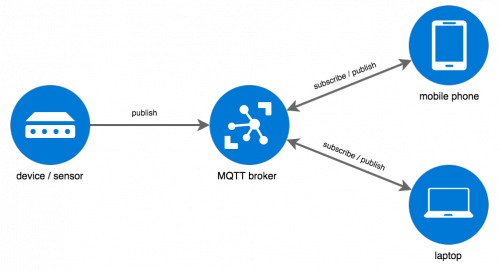
\includegraphics[width=0.9\textwidth]{MQTT.png}
	\caption{MQTT Architecture with the broker in the middle as a mediator between the clients.\cite{2018-11-24Pure-javascript-MQTT-broker}}
	\label{MQTT}
\end{figure}

REST is an architectural paradigm describing how distributed systems can communicate with each other. It consists of five mandatory and one optional restriction. If any of the five mandatory restrictions are violated, an architecture cannot be RESTful. The restrictions are 
\begin{enumerate}
    \item Client–server architecture
    \item Statelessness
    \item Cacheability
    \item Layered system
    \item Uniform interface
    \item Code on demand (optional)
\end{enumerate}
REST was developed by Roy Fielding alongside to HTTP/1.1 and although is not dependent on it, is the primary used protocol to implement REST. Thus, many web pages fulfill these restrictions naturally. REST messages are usually human readable JSON files. Unlike MQTT, REST does not rely on a broker.  \cite{Fielding2000ArchitecturalArchitectures} \newline

For many cases in the past it was hard for the maintainers to adhere to all REST principles due to its strict nature. Moreover, REST is usually implemented with HTTP/1.1. In 2015 HTTP/2 was released to adress the flaws of its predecessor. \cite{SayfanLastvisited2018-11-242018RESTAPIs} Among those are the lack of ability of constant data streaming, latency issues etc. gRPC fully takes advantage of HTTP/2 and thus has some advantage over REST. It uses stubs to describe an interface. Stubs are independent of any programming language. Unlike in most implementations of REST, gRPC does not use textual transport data like JSON but relies on Protobuf, a binary buffer. Moreover, Google offers an \textit{Extensible Server Proxy} (ESP), which offers a transcoding from HTTP/JSON to gRPC. \cite{2018-11-242017Grpc-gateway, Lastvisited2018-11-272018CloudGRPC} \newline

\begin{figure}[ht]
	\centering
  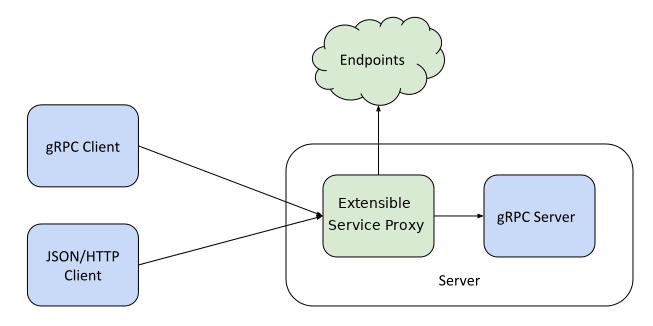
\includegraphics[width=0.7\textwidth]{gRPC_ESP.png}
	\caption{Deployed endpoints gRPC application. \cite{Lastvisited2018-11-272018CloudGRPC}}
	\label{ESP}
\end{figure}

GraphQL is a data query and -manipulation language. It was developed by Facebook and is open source since 2015. Compared to REST it is has a more flexible and efficient approach. Increase in efficiency over REST is based on faster mobile data access, and more flexibility for the API to let clients access precisely the data it needs,  i.e. the server modifies the data with respect to the clients needs instead of providing one rigid resource. \cite{LastVisited2018-15-122018BasicsIntroduction} 

OPC UA Vision is a companion specification adressing robotics and object detection. \cite{VDMA2018OPCSpecification} It's scope is to standardize the interfaces between the machine vision system and its process environments. A possible use case would be a conveyor belt that should be halted if any higher system level tells it to do so. Then, image acquisition can conducted by the machine vision system. As soon as image acquisition is done, an event should be fired which tells the higher production system the result of the acquisition. The conveyor belt can then continue. In June 2018 the first part of OPC UA Vision was released. This parts includes the basic skills on the infrastructure layer, such as result transmission, machine status etc. The following parts which have not been released yet should include machine vision skills such as post detection or a completeness check. As of now, there is no implementation of OPC UA Vision available and thus can only be used on an conceptual level.

\section {Deployment Options}
\label{deploymentoptions}
In the last decade, most applications had a monolithic character which did not focus much on scalability and interfaces. With the progress in digitalization, applications had to become more flexible and faster. To address this problem, the container architecture came about. Unlike a virtual machine which needs an operating system, runtime, system variables etc. to operate well, docker and others are sandbox systems which can imply all the mentioned features and furthermore can run on almost any operating system. See figure \ref{container} for an illustration. In the following, two possible deployment options are discussed, namely Heroku and Docker.\cite{WurbsLastvisited2018-11-272017DockerVeraendern}

\begin{figure}[ht]
	\centering
  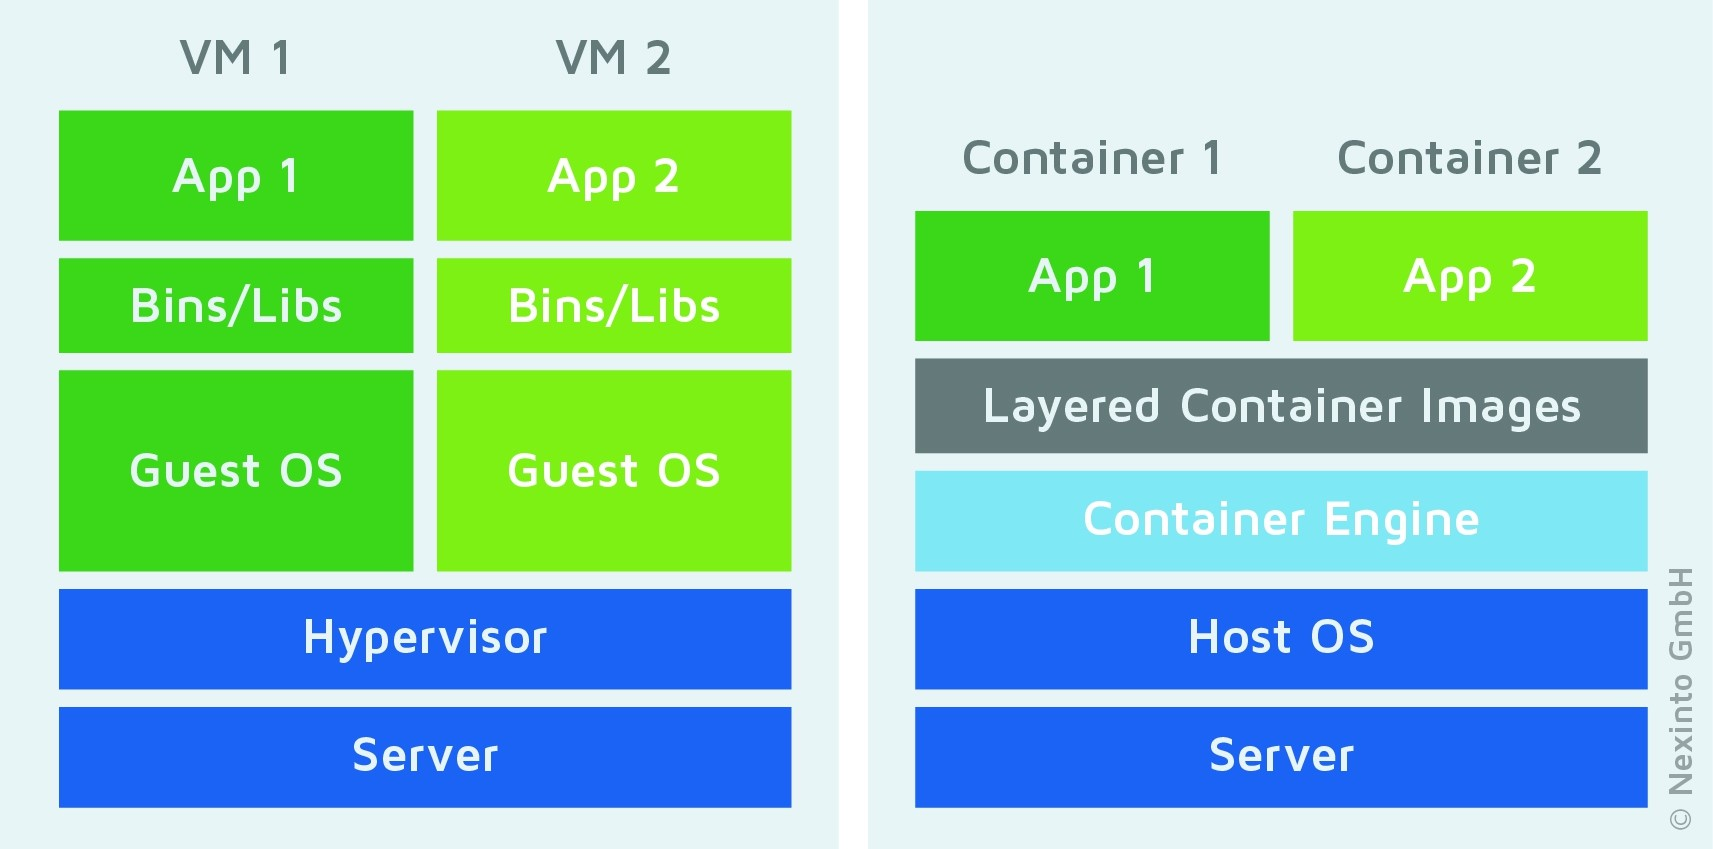
\includegraphics[width=0.7\textwidth]{containervsvm.jpg}
	\caption{Virtual machine architecture on the left versus container architecture on the right. Docker does not rely on a hypervisor.\cite{WurbsLastvisited2018-11-272017DockerVeraendern}}
	\label{container}
\end{figure}

Docker is an open source standard for operating-system-level virtualization. If docker is installed on an operating system, it is possible to run several apps on the machine simultaniously, with low start and stop times and little overhead. In combination with a continuous integration and continuous delivery platform, development and operations can be harmonized.

Heroku is a platform as a service provider which underlying technology shares some core concepts with Docker. E.g. BuildPacks are a set of scripts which are used to setup the final state of an image. The pendant on the Docker side is called Dockerfile. See \cite{ThurigLastvisited2018-27-112014DockerHeroku} for a full description of the similarities and \ref{dockerandheroku} for a list of pendants. However, there are also differences for the two alternatives. The main one is the dependency on the Heroku platform on the Heroku side, whereby on the Docker side one is completely flexible to choose any environment from Raspberry Pi to cloud platform providers like Amazon Web Services. This also means a surplus of workload on infrastructure on the Docker side. Also, one is less flexible on the prices. Heroku has a staged price model ranging from 0 to 500\,\$ per month and dyno. Docker is again more flexible in letting one just paying for the hosting and storaging and leaving the additional features provided by Heroku aside. \cite{ChrisLastvisited2018-11-272017WhyDocker} 


\begin{table}
\begin{center}
      \caption{Similar core concepts of Docker and Heroku. \cite{ThurigLastvisited2018-27-112014DockerHeroku}}
  \begin{tabular}{ l | l }
    Docker & Heroku  \\ \hline
Dockerfile &	BuildPack \\ 
Image	& Slug\\ 
Container&	Dyno\\ 
Index	&Add-Ons\\ 
CLI	&CLI
  \end{tabular}
  \label{dockerandheroku}
\end{center}
\end{table}

\section{Service Oriented Architectures}